\chapter{Heuristics}
As the number of nodes in a problem increases, the execution of exact algorithms becomes increasingly computationally demanding. Consequently, heuristic algorithms are employed, which do not guarantee an optimal solution but provide a satisfactory one with reasonable computational cost. We will introduce two families of heuristics:

\begin{itemize}
    \item \textbf{Constructive heuristics}: Generate an approximate solution from scratch.
    \item \textbf{Refinement heuristics}: Improve an existing solution.
\end{itemize}

Constructive heuristics build a solution in a feasible amount of time, typically achieving within 15-20\% of optimality. These heuristics are often used as a starting point for other heuristics, as the quality of the final solution heavily depends on the initial instance.

\section{Nearest Neighbors}
This constructive heuristic algorithm is a greedy 2-approximation algorithm, meaning that the solution is at most 100\% away from the optimum. It generates a solution for the TSP instance in \(O(n^2)\) time, starting from one node and selecting the next node in the tour that is closest to the current node at each iteration \cite{article} \cite{inproceedings}. The step of this algorithm are the following:

\begin{enumerate}
    \item Select a random node.
    \item Find the nearest unvisited node and go there.
    \item If there are any unvisited nodes left, repeat step 2.
    \item Return to the first node.
\end{enumerate}

The pseudocode for computing a single starting solution from an arbitrary node is shown in Algorithm~\ref{alg:NN_algo}.\\

\begin{algorithm}
    \caption{Nearest Neighbour}
    \label{alg:NN_algo}
    \begin{spacing}{1.2} % Adjust this value to change line spacing
        \KwIn{Starting node}
        \KwOut{A valid tour}
        \BlankLine
        path $\leftarrow \{\}$\;
        current\_node $\leftarrow \{first\_node\}$\;
        visited $\leftarrow \{first\_node\}$\;
        solution $\leftarrow 0$\;
        \While(\tcc*[f]{While there are unvisited nodes}){$|visited| \neq N$}
        {
            closest\_node $\leftarrow $ nearest node \KwTo $current\_node \notin$ visited\;
            solution $\leftarrow solution$ $+$ $dist(closest\_node$, $current\_node)$\;
            current\_node $\leftarrow closest\_node$\;
            \textbf{add} $current\_node$ \KwTo $visited$\;
            \textbf{add} ($current\_node$, $closest\_node$) edge \KwTo $path$\;
        }
        \textbf{add} ($current\_node$, $first\_node$) edge \KwTo $path$\;
        $solution \leftarrow solution $ $+$ $dist(first\_node$, $current\_node$)\;
        \BlankLine
    \end{spacing}
\end{algorithm}

Despite its simplicity and speed of implementation, this algorithm often find suboptimal solutions. However, these limitations can be mitigated using improvement techniques such as the 2-opt algorithm, which further enhances the quality of the obtained solution.

\newpage

\subsection{Nearest Neighbors from each node}
An enhanced version of the algorithm can be developed by initiating the process from each possible node. This adjustment brings the complexity to \(O(n^3)\), which is still significantly more efficient than the exponential complexity of exact algorithms. This modification mitigates the algorithm's sensitivity to initial conditions, thereby increasing its robustness. The pseudocode for this enhanced approach is as follows Algorithm~\ref{alg:NN2_algo}:

\begin{algorithm}
    \caption{Nearest Neighbour From Each Node}
    \label{alg:NN2_algo}
    \begin{spacing}{1.2} % Adjust this value to change line spacing
        \KwIn{TSP istance}
        \KwOut{A valid tour}
        \BlankLine
        path $\leftarrow \{\}$\;
        \ForEach{node n}
        {
            current\_path $\leftarrow NearestNeighbors(first\_node\=n)$\;
            \BlankLine
            \If{current\_path \textbf{better than} path}{
                path $\leftarrow current\_path$\;
            }
        }
        \BlankLine
    \end{spacing}
\end{algorithm}

\section{Refinement Heuristics with 2-Opt}
Once a tour has been generated by a construction heuristic, it can be improved using methods like the 2-opt local search. This kind of heuristic starts from a given solution and improves it by making small changes. Their performances are strongly dependent on the construction heuristic used. Other metaeuristics methods to enhance the solution include tabu search \ref{chap:tabusec} and simulated annealing, both of which utilize the 2-opt move to find neighboring solutions.

This heuristic proposed in 1958 by G. A. Croes \cite{2opt}, first use some construction algorithm and then iteratively improves this tour by resolving crossing edges (\ref{fig:crossing_edge}). This is done by selecting an edge \((e_1, e_2)\) and searching for another edge \((e_3, e_4)\), completing a move only if:

\[ \text{dist}(e_1, e_2) + \text{dist}(e_3, e_4) > \text{dist}(e_2, e_3) + \text{dist}(e_1, e_4) \]

\begin{figure}[H]
    \centering
    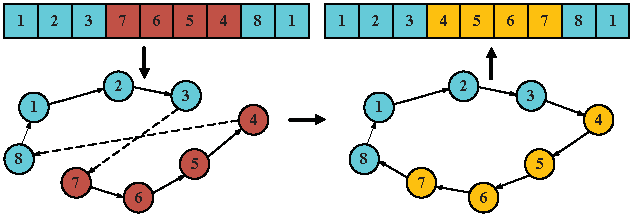
\includegraphics[width=0.9\linewidth]{Immagini/Crossing edges.pdf}
    \caption{Illustration of the process for removing an intersection in a path.}
    \label{fig:crossing_edge}
\end{figure}

This ensures a valid tour, as shown in Figure~\ref{fig:2opt_before_after}. The process continues until no more 2-opt improvements can be found, resulting in a 2-optimal tour. \\

\begin{figure}[H]
    \centering
    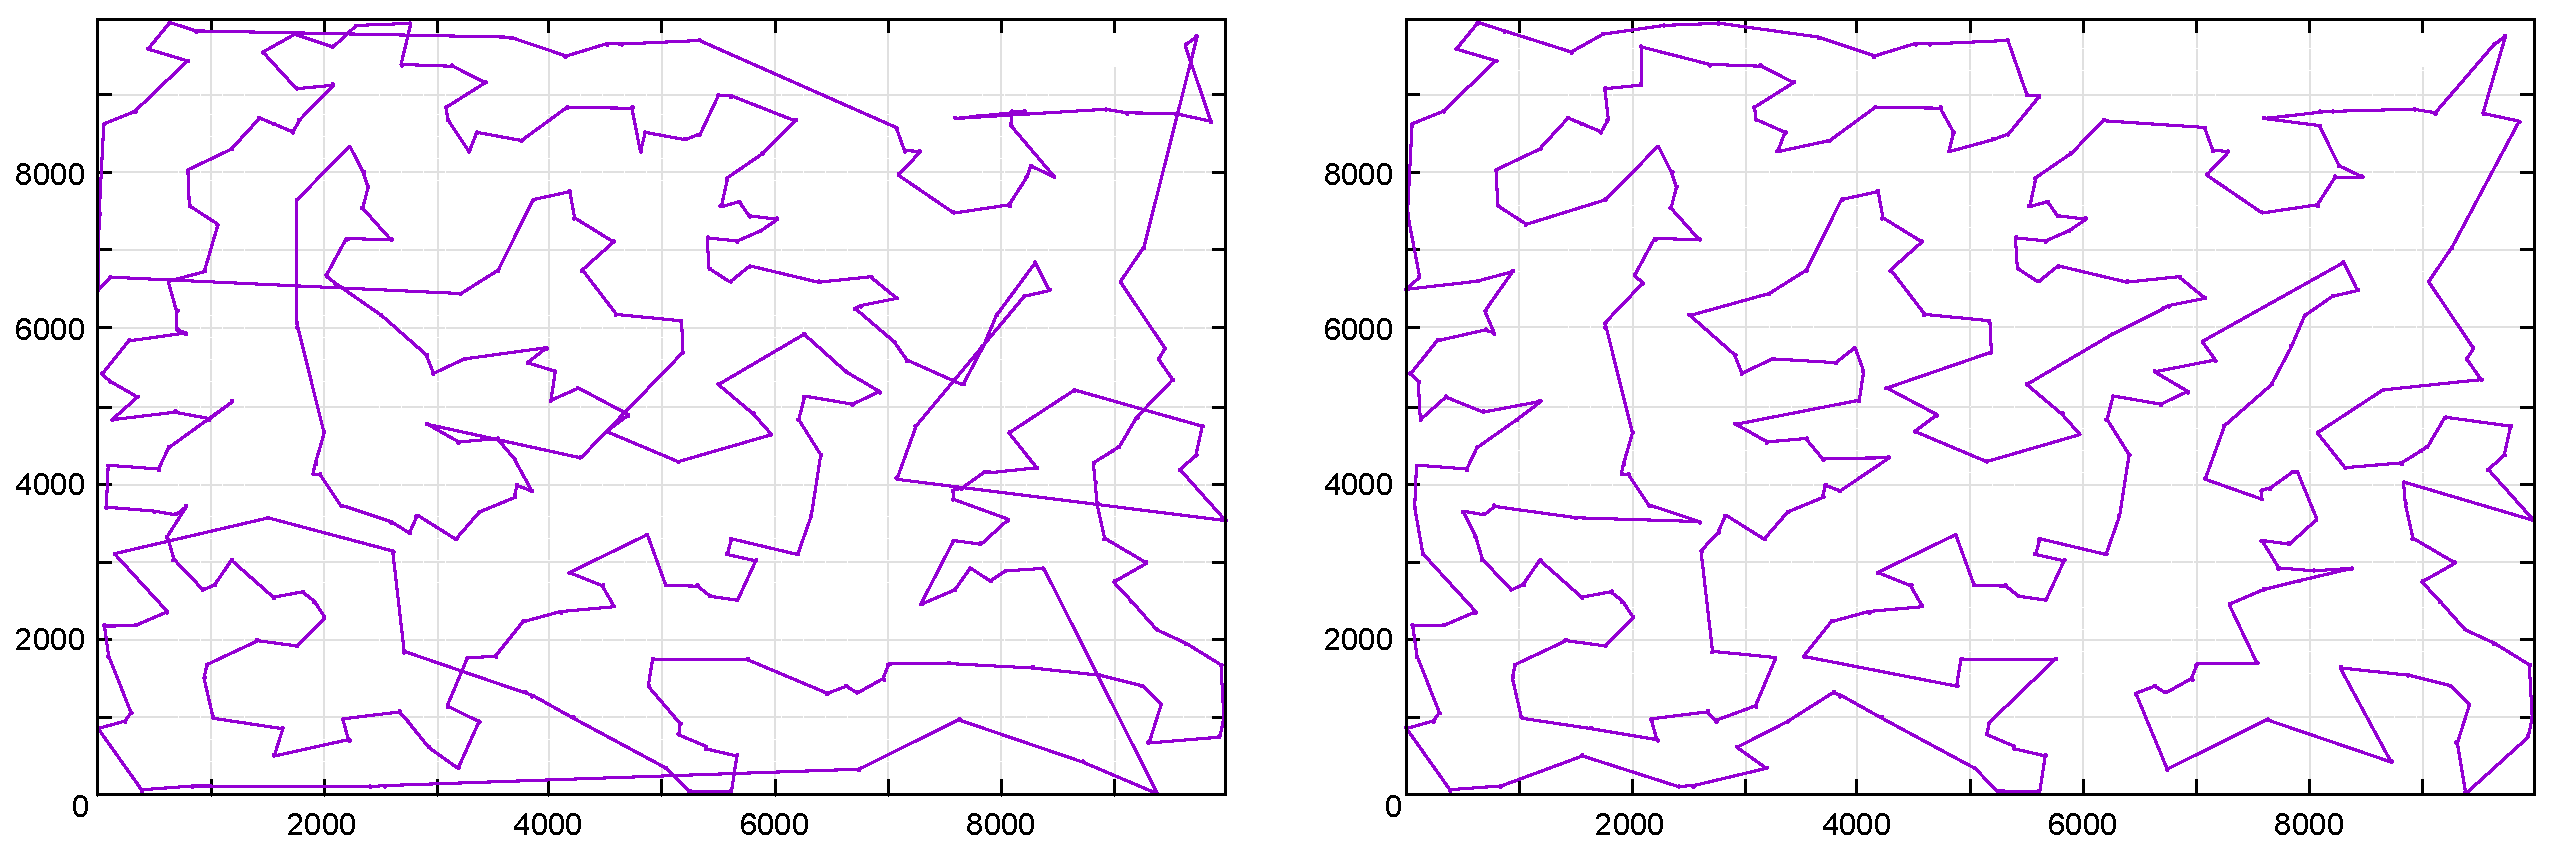
\includegraphics[width=\linewidth]{Immagini/NN+2opt.pdf}
    \caption{2-opt before (left) and after (right)}
    \label{fig:2opt_before_after}
\end{figure}

% \begin{figure}[htbp]
%     \centering
%     \begin{subfigure}[b]{0.48\textwidth}
%         \centering
%         \includesvg[width=\textwidth]{Immagini/svg/NN.svg}
%         \caption{Before}
%         \label{fig:2opt_before}
%     \end{subfigure}
%     \hfill
%     \begin{subfigure}[b]{0.48\textwidth}
%         \centering
%         \includesvg[width=\textwidth]{Immagini/svg/NN+2opt.svg}
%         \caption{After}
%         \label{fig:2opt_after}
%     \end{subfigure}
%     \caption{2-opt before and after}
%     \label{fig:2opt_before_after}
% \end{figure}

\newpage

\noindent The 2-OPT algorithm is shown in Algorithm~\ref{alg:2OPT_algo}.

\begin{algorithm}[H]
    \caption{2-Opt}
    \label{alg:2OPT_algo}
    \begin{spacing}{1.3}
        \KwIn{A valid tour}
        \KwOut{An optimized valid tour}
        \BlankLine
        counter \leftarrow $0$\;

        \While{counter < \#nodes \textbf{and} time < time\_limit}
        {
            counter \leftarrow $counter + 1$\;

            A \leftarrow $tour[0]$\;
            A1 \leftarrow $tour[1]$\;
            \BlankLine
            \For{B \textbf{from} $tour[2]$ \textbf{to} $tour[-2]$}
            {
                B1 \leftarrow $B + 1$\;

                $\Delta(A,B) \leftarrow (c_{A,B} + c_{A1,B1}) - (c_{A,A1} + c_{B,B1})$\;
                \BlankLine
                \If{$\Delta(A,B) < 0$}
                {
                    \tcc{Reverse subvector from A1 to B}
                    \textbf{reverse subvector} $tour[A1 : B]$

                    tour.cost \leftarrow $tour.cost$ + $\Delta(A,B)$

                    \If{current solution better than official solution}
                    {
                        update official solution\;
                    }
                }
            }
            \BlankLine
            move A to the end of the array\;
        }
        \BlankLine
    \end{spacing}
\end{algorithm}

\newpage

\section{Comparison between Heuristics}
As shown in Figure \ref{fig:2opt_before_after}, the result can vary significantly in terms of route and therefore cost, as all possible intersections are eliminated thanks to the 2-opt method, as previously mentioned. However, this may in turn lead to an increase in processing time to remove the intersections and find a better route, in particular with large input files.

Figure \ref{fig:NN_2opt} illustrates the performance profile with the cost comparison between the Nearest Neighbor and the Nearest Neighbor with 2-opt. We can see that the 2-opt gives better result, with an error less the 10\% in every class, while the Nearest Neighbor alone reaches a 20\% in most cases.

\begin{figure}[H]
    \centering
    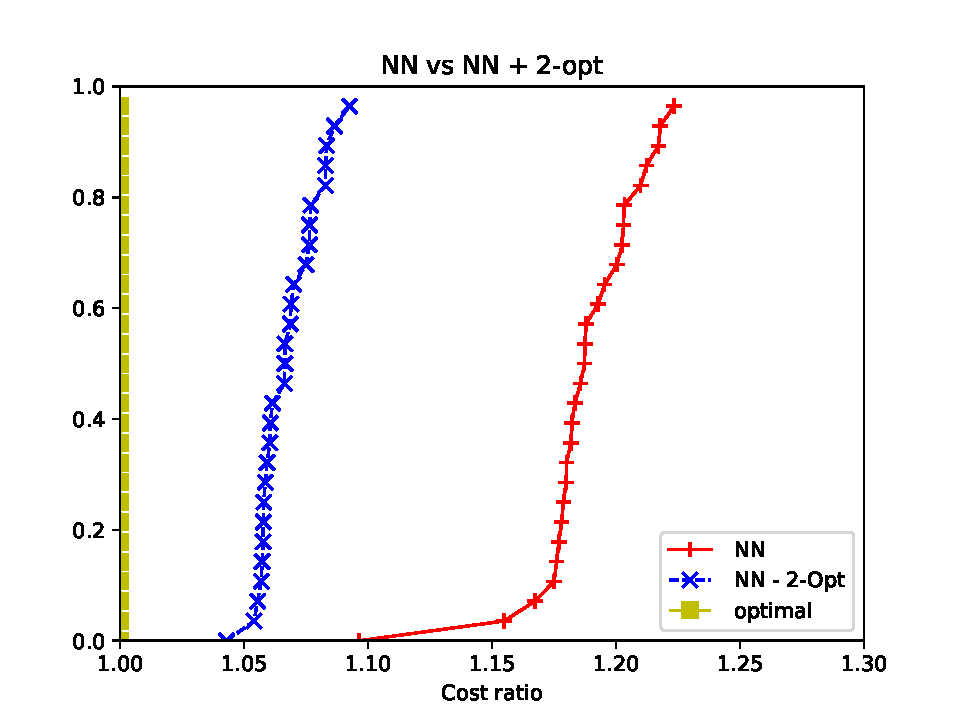
\includegraphics[width=0.7\linewidth]{Immagini/NN vs 2Opt.pdf}
    \caption{Performance Profile of Nearest Neighbor and Nearest Neighbor with 2-opt.}
    \label{fig:NN_2opt}
\end{figure}
